% vim: set filetype=tex spell :

%CubeSat Chapter 
\chapter{CubeSat Hardware Implementation}

\label{ch:CubeSatHardware}

\section{CubeSat Architecture}

\todo[inline]{Float section to background?}

The \ac{ARC} uses the same board geometry as the CubeSat Kit\cite{CSK} hardware making it compatible with other CubeSat hardware. The \ac{ACDS} board has a slightly different shape than the standard board shape to accommodate the torquers.

\subsection{Stackup}

\Cref{fig:arcMech} shows the mechanical design of the \ac{ARC}. The design has a central board stack with solar pannels and rails attached to rings that are on the top and bottom of the board stack. The \ac{ACDS} board is located 3rd from the bottom of the stack. This puts it in the center of the board stack. Because the solar cells cover all of the side faces except a small strip in the center this makes the \ac{ACDS} board the only place to put access port connections. The separation switch connections are also located on the \ac{ACDS} board as the separation switch is attached to one of the torquer standoff.

\begin{figure}[!ht]
    \centering
    \begin{minipage}{0.41\linewidth}
        \begin{tikzpicture}[remember picture] 
            \def\sysx{1.8}
            \pgftext{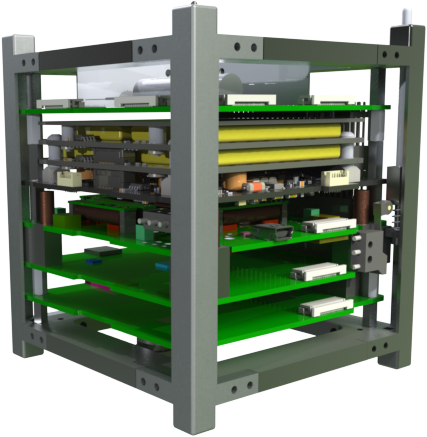
\includegraphics[width=\linewidth]{cubesat-core}}
            % define destination coordinates
            \path (\sysx,1.76) coordinate (LEDL)
                  (\sysx,0.85) coordinate (EPS)
                  (2.4,0.2) coordinate (Z1tq)
                  (-2.5,0.39) coordinate (Z2tq)
                  (-1.28,0.1) coordinate (Xtq)
                  (\sysx,-0.27)  coordinate (ACDS)
                  (\sysx,-0.96)  coordinate (COMM)
                  (\sysx,-1.55)  coordinate (IMG);
        \end{tikzpicture}
    \end{minipage}\begin{minipage}{0.22\linewidth}
        \begin{itemize}
            \itemsep-0.3em
            \item[\kern-2em] \tikz[na] \coordinate (LEDLi); LEDL
            \item[\kern-2em] \tikz[na] \coordinate (EPSi); EPS
            \item[\kern-2em] \tikz[na] \coordinate (Ztqi); Z Torquer
            \item[\kern-2em] \tikz[na] \coordinate (Xtqi); X Torquer
            \item[\kern-2em] \tikz[na] \coordinate (ACDSi); ACDS board
            \item[\kern-2em] \tikz[na] \coordinate (COMMi); COMM
            \item[\kern-2em] \tikz[na] \coordinate (IMGi); IMG
        \end{itemize}
    \end{minipage}

    \begin{tikzpicture}[overlay,remember picture]
            \path[->,red,very thick] (LEDLi) edge (LEDL);
            \path[->,red,very thick] (EPSi) edge (EPS);
            \path[->,red,very thick] (Ztqi) edge (Z1tq);
            \path[->,red,very thick] (Ztqi) edge (Z2tq);
            \path[->,red,very thick] (Xtqi) edge (Xtq);
            \path[->,red,very thick] (ACDSi) edge (ACDS);
            \path[->,red,very thick] (COMMi) edge (COMM);
            \path[->,red,very thick] (IMGi) edge (IMG);
    \end{tikzpicture}
    \caption{The \acs{ARC} mechanical setup}
    \label{fig:arcMech}
\end{figure}

\subsection{Mechanical Considerations}
In addition to the \ac{ACDS} hardware the \ac{ACDS} board also contains the pull pin and USB connection. This is located on the \ac{ACDS} board because it is the only board that can connect to the access port. The pull pin and USB connection connect directly to the header and are not connected to the core \ac{ACDS} hardware. 

The Z-axis torquers are housed inside the standoffs which are located on the four corners of the board. To accommodate the torquers notches are cut out of the \ac{ACDS} board. This is visible in \cref{fig:layout}. The notches are designed to fit the torque standoffs and help keep them in the proper orientation. The torquers fit into a hole drilled into the standoffs and are healed in place with epoxy. 


\subsection{Bus Communication}

The subsystems of the \ac{ARC} will communicate with each other using the ARCBus. The ARCBus consists of shared connections between the subsystems to transmit commands and data. The ARCBus will primary used by the \ac{ACDS} to get sensor data from the \ac{LEDL} and send and receive data to the ground station through the COMM system. Commands are transmited using an \ac{I2C} bus and large blocks of data are sent using a SPI bus which is negotiated using the \ac{I2C} bus.

\section{\acl{ACDS} System Block Diagram}

The block diagram for the CubeSat hardware used to implement the \ac{ACDS}. The hardware necessary for the \ac{ACDS} is spread over multiple subsystems of the \ac{ARC}. The \ac{ACDS} board contains the torquers, driving hardware along with the microcontroller which will run the attitude control algorithm. There is one two axis magnetometer located on each of the six of the \acp{SPB}. These are used by the \ac{ACDS} to calculate rotation rates and calculate the magnetic dipole moment required to generate the necessary torque. Spreading the magnetometers across all six faces should give some degree of noise immunity and redundancy. The \ac{LEDL} board also contains \ac{MEMS} angular rate sensors as a redundant reading of the rotation rate of the \ac{ARC}. The sensors on the \acp{SPB} are read by the \ac{LEDL} which then forwards the magnetometer and angular rate measurements to the \ac{ACDS}.

\begin{figure}[H]
    \centering
    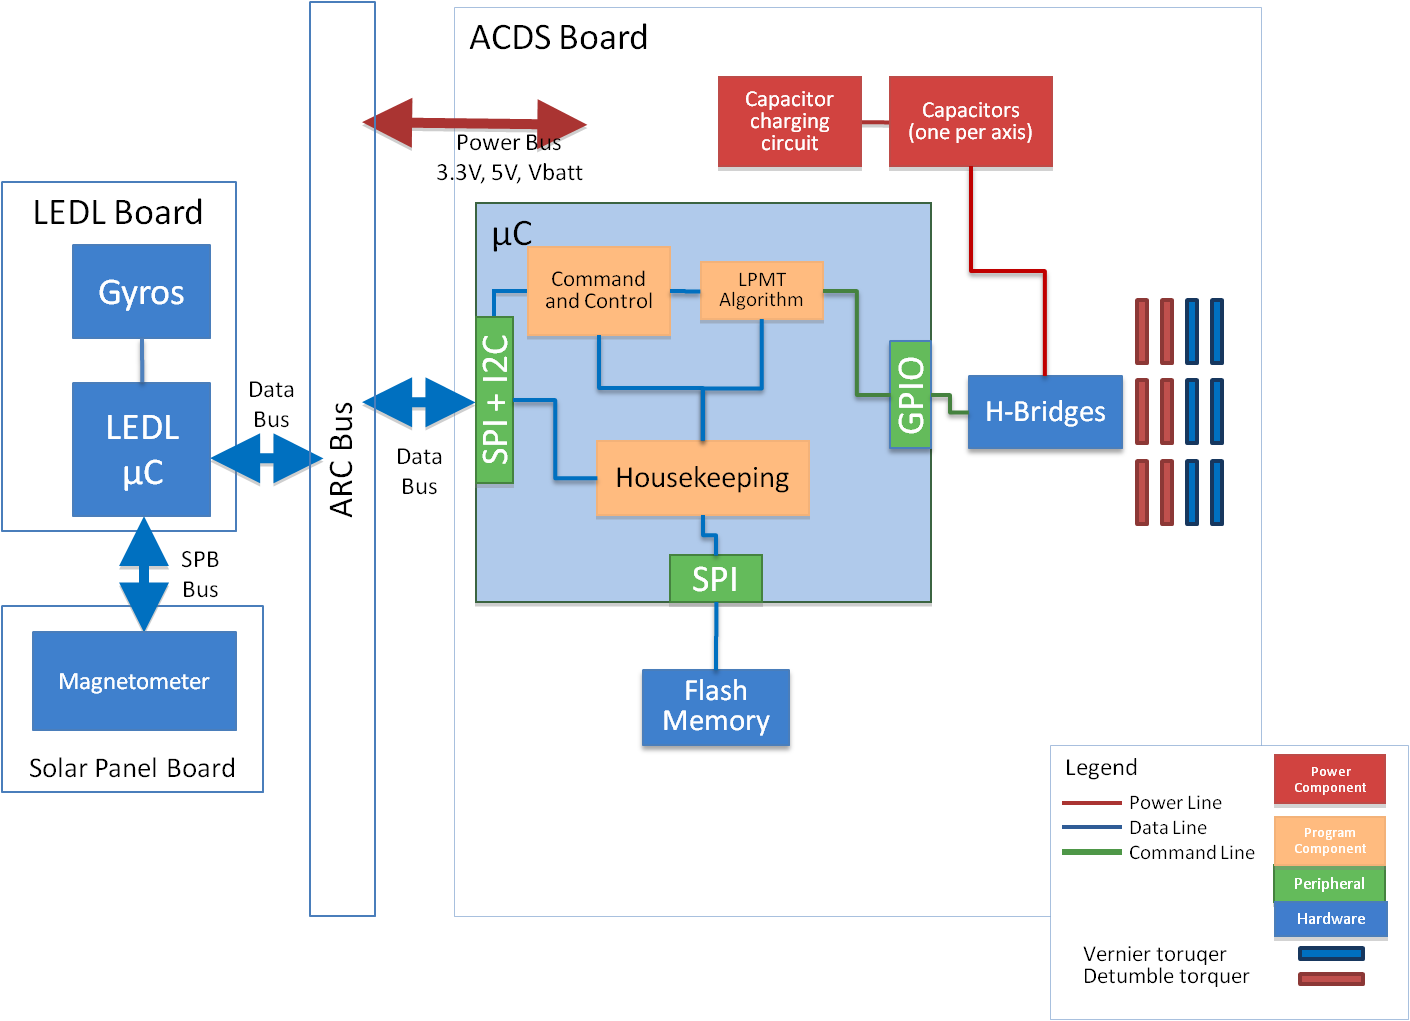
\includegraphics[width=0.8\textwidth]{Figures/Block}
    \caption{Block Diagram of the CubeSat \acs{ACDS} system}
\end{figure}


\section{Torquers}

The torquers for the CubeSat consist of a hard magnetic core surrounded with a coil of wire. The torquers are flipped using the driving circuit which causes a current pulse to flow through the coil.

\subsection{Cores}

The torquer cores from \cite{Mentch11} consisted of a large and a small pair in each axis. The torquers consist of a hard magnetic core an electromagnetic coil to flip the core. All torquer cores were the same size, one inch long $\sfrac{1}{16}$th inch diameter rod. The large pair was made of Alnico1 and produced a magnetic dipole moment of $0.022 \unit{A m^2}$. The small pair was proposed to have an inert core with a thin permalloy coating to give it a dipole moment of $0.00011 \unit{A m^2}$.

The torque that the alnico torquers produce is quite small and is already not easy to measure. Because the small torquers are $\sfrac{1}{200}$th the size of the alnico torquers it was determined that these are not feasible to fabricate. To fix this the small torquers was enlarged to 10\% of the size of the large torquers. The switching interval was also reduced to one second. It was also necessary to relax the desired attitude tolerances to accommodate the new setup.

\subsection{Coils}

The torque coils are the same for both the large and small torquers. The coils consist of four layers of 26 AWG wire.

\subsection{Drivers}

The schematic to drive a pair of torquers is shown in \cref{fig:drive}. Each pair of torquers is driven by three complimentary pairs of \acp{MOSFET}.  The \acp{MOSFET} are driven by three pairs of \ac{MOSFET} drivers which are controlled by the \ac{ACDS} microcontroller.

In the idle state all of the \acp{MOSFET} are off and the torquer coils are floating. This prevents changing magnetic fields in the torquers causing current to flow in them. To flip a torquer one end of the torquer is shorted to ground using one of the N-Channel \acp{MOSFET} and the other end is shorted to C1 using one of the P-Channel \acp{MOSFET}. After a short delay the \acp{MOSFET} are switched off and C1 begins to recharge.

\begin{figure}[H]
    \centering
    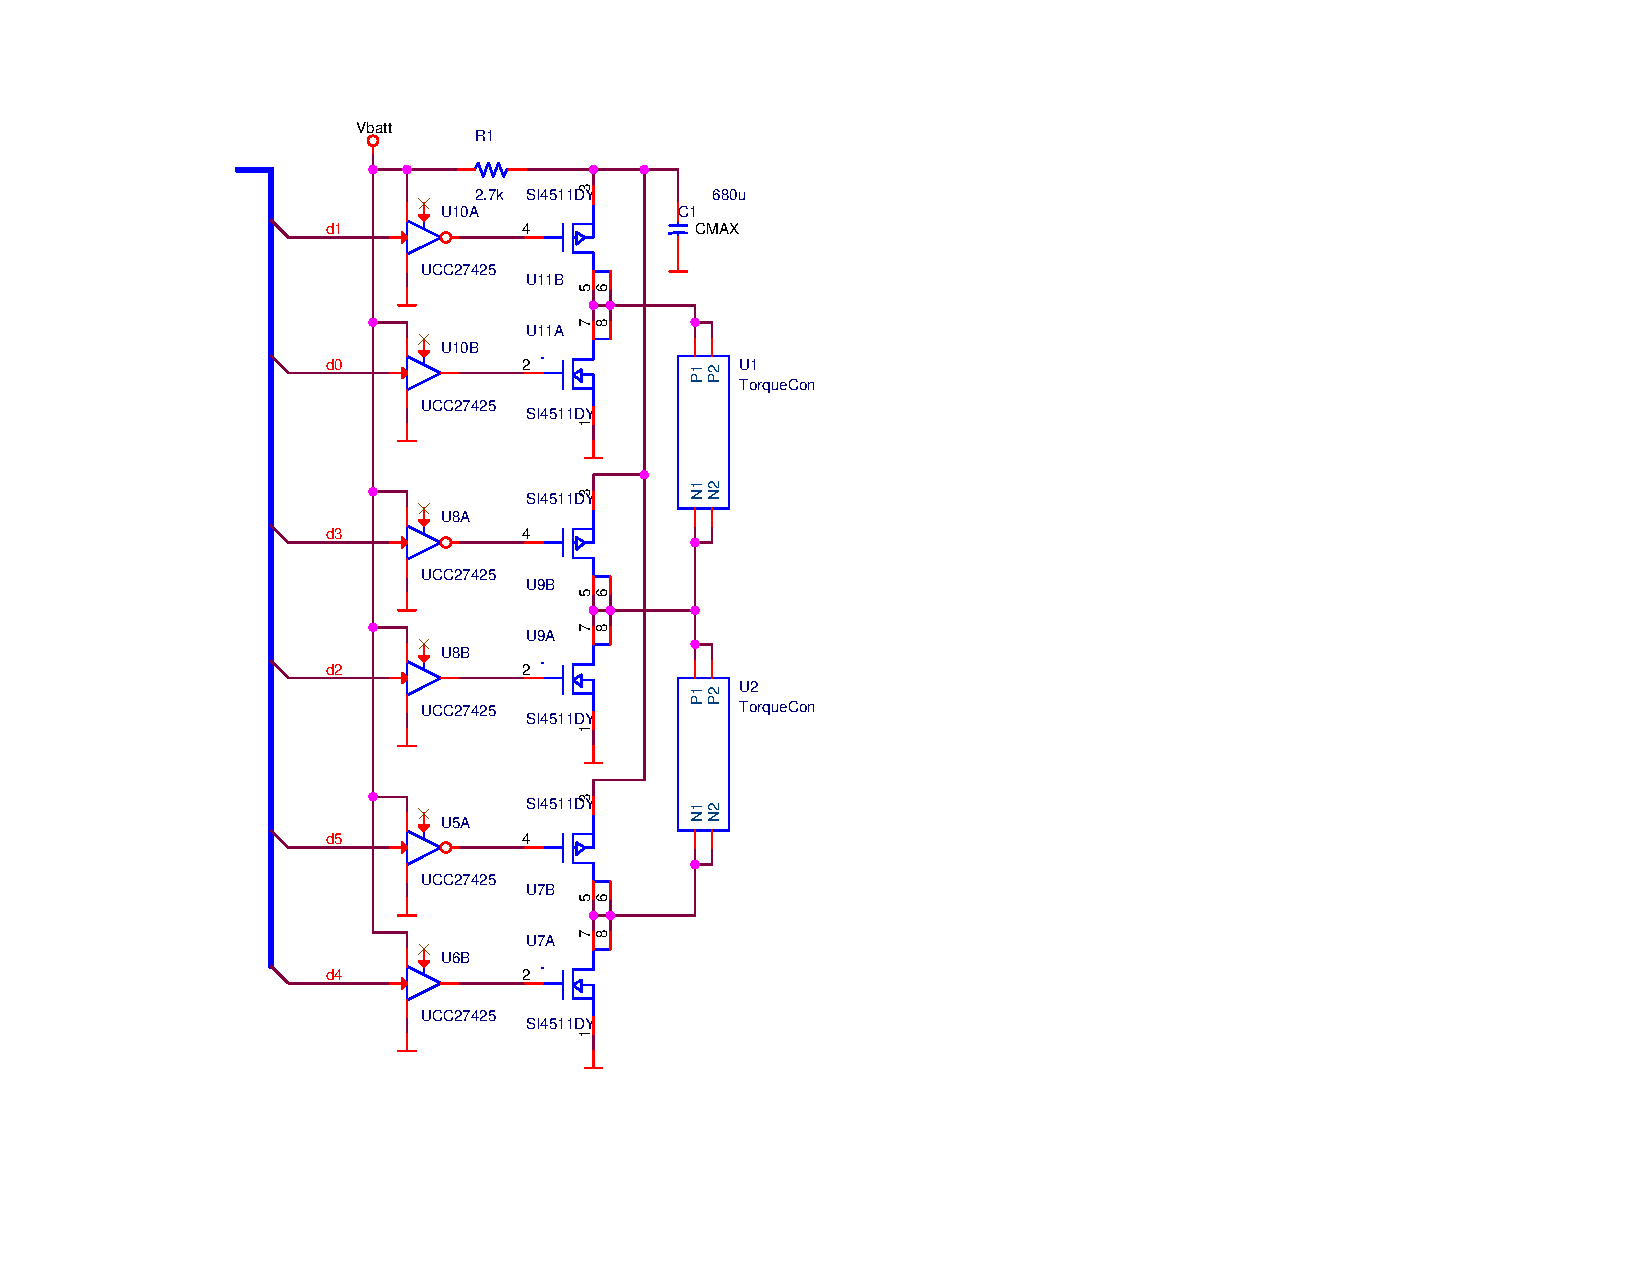
\includegraphics[width=0.5\textwidth]{Figures/driverSchematic}
    \caption{Torquer Driver schematic}
    \label{fig:drive}
\end{figure}

\subsection{Torquer Diagnostics}

Comparators are used to detect in flight if the torquers and drivers are functioning properly. One comparator is used to determine if the capacitor is charged and another is used to detect if the capacitor is discharged. The comparators are checked both before and after a torquer flip to see if the capacitor was charged before an attempted flip and discharged after. If the capacitor did not discharge then the torquer did not flip probably because of a bad connection somewhere. This information is logged in flight and can be used on the ground to analize how well the torquers are working.

\todo[inline]{Need some discussion of what is done with the info but also need to figure out what should be done.}


\section{Sensors}

The only sensor called out in \cite{Mentch11} was a magnetometer. The accuracy of the magnetometer was not specified but it needs to be able to determine rotation rates accurately enough for the \ac{ACDS} to work.

\subsection{Magnetometer}

The magnetometers on the satellite are Honeywell HMC1052 \ac{AMR} sensors. These sensors use \ac{AMR} elements in a bridge configuration to measure the field in each axis. The HMC1052 is a 2-axis sensor that measures the field in the axis that are parallel to the board that it is mounted on (X and Y). Each face of \ac{ARC} will have a single HMC1052 giving a total of 4 measurements in each axis.

\subsubsection{Magnetometer Amplifier}

\todo[inline]{This is mostly for my reference. Should it be here?}

The \ac{SPB} also contains an amplifier to amplify the magnetometer signal before it is read by the \ac{ADC}. This allows the output voltage of the magnetometer to fill the input range of the \ac{ADC}. The required range of the magnetometer will be largely dependent on the torquer geometry and could be more then the $\pm$600 mGuass or so of earths field. The amplifier can be used to trade range for resolution depending on what is needed.

The gain for the amplifier can be calculated as follows: If the maximum output range of the sensor is restricted to $\pm$ 4 gauss. With a bridge voltage of 3.3 V and a sensitivity of 1 mV/V/gauss this results in a $\pm$ 13.2 mV voltage swing. The bridge offset is $\pm$ 1.25 mV/V or $\pm$ 4.125 mV. This results in a total possible swing of $\pm$ 17.325 mV. The input voltage range of the \ac{ADC} is $\pm$ 1.65 V. This results in a gain of about 95. 

\subsubsection{Magnetometer \acl{ADC}}

Each magnetometer has its own \ac{ADC} on each \ac{SPB}. The \ac{ADC} used is the LTC2487. The LTC2487 is a 16-bit delta sigma \ac{ADC} that has two differential analog input channels and an \ac{I2C} interface. For a bridge voltage of 3.3V the HMC1052 has a sensitivity 3.3mV/Gauss. If the amplifier gain is 95 this results in a sensitivity of 0.31V/gauss. For a 3.3V reference voltage the \ac{ADC} has a resolution of $25 \mu V$ this results in a resolution of 81 $\mu$Gauss / LSB.

\subsubsection{Magnetometer Operation}

\todo[inline]{Background or Appendix?}

The \ac{AMR} sensors are primarily sensitive to magnetic fields in their sensitive direction but they are also slightly sensitive to magnetic fields in an axis normal to the sensitive direction. The sensor is only sensitive to magnetic fields that are in the film plane, which is the plane that the \ac{AMR} film is deposited in. For the 2-axis HMC1052 this means that both sensors show some sensitivity to fields in both the X and Y axes. The cross axis effect varies from sensor to sensor \todo{Test this} so calibration values must be calculated for each sensor \cite{AN215}.

\Cref{eq:magfull} shows the full equation for the magnetometer. $V_b$ is the bridge voltage that is applied to the sensor. $S_s$ is the sensitivity in the sensitive direction. C and D are the cross field sensitivity and offset values \cite{AN215}.

\begin{equation}
    V_o = V_b \left( \left( S_s \left( 1 + C \cdot H_c^2 \right) H_s \right) + D \cdot H_c \right)
    \label{eq:magfull}
\end{equation}

Because C is small and is multiplied by miligauss squared to get a really small number, it is ignored for the purposes of calibration which results in the simpler \cref{eq:magcross}.

\begin{equation}
    V_o = V_b \left( \left( S_s H_s \right) + D \cdot H_c \right)
    \label{eq:magcross}
\end{equation}

\Cref{eq:magcross} is useful to determine the voltage that would be produced for a given magnetic field condition, but not terribly useful if the sensor voltages are known but the fields are not. Furthermore the \ac{ADC} reference voltage will be the same as $V_b$ so knowing the bridge voltage is unnecessary\todo[prepend, caption={Elaborate Here?}]{Seems more or less obvious to me and somewhat cumbersome to fully explain}. 
 
\begin{equation}
    H = C_1 \cdot V_x + C_2 \cdot V_y + C_3
    \label{eq:magcal}
\end{equation}

Because $S_s$ and D from \cref{eq:magcross} are experimentally determined, it is easier to solve \cref{eq:magcal} for calibration instead. In this case $V_x$ and $V_y$ are the \ac{ADC} values for the x and y axis respectively. $C_1$ and $C_2$ are the sensitivity and $C_3$ is an offset that can come from offsets in the instrumentation or from external offsets such as torquers. This makes the values that the calibration solves for directly usable to calculate magnetic field from \ac{ADC} measurements.

\subsubsection{Magnetometer Calibration}

Magnetometer Calibration consists of finding the coefficients in \cref{eq:magcal}. To do this the magnetometer is first placed inside the Helmholtz Cage. This allows the field to be set to any value. Furthermore the field can be set under Matlab control so the entire calibration process can run automatically. The calibration program sweeps the field inside the Helmholtz Cage through a predefined sequence and reads the sensor output at each point. 

\vspace{2em}
\todo[inline]{Move to background/appendix?}
\Cref{eq:magcal} can be rearranged into matrix form as shown in \cref{eq:magmat}. Each line in the matrix represents a separate magnetic field measurement. H is the value set by the Helmholtz cage in the sensitive axis . 

\begin{equation}
    \vect{b}=\matt{A} \vect{x} \quad
    \matt{A} =
    \begin{bmatrix}
        {V_x}_1 & {V_y}_1 & 1 \\
        \vdots & \vdots & \vdots\\
        {V_x}_n & {V_y}_n & 1 \\
    \end{bmatrix} \quad
    \vect{x} = 
    \begin{bmatrix}
        C_1 \\
        C_2 \\
        C_3 \\
    \end{bmatrix} \quad
    \vect{b} = 
    \begin{bmatrix}
        H_1 \\
        \vdots \\
        H_n \\
    \end{bmatrix} \quad
    \label{eq:magmat}
\end{equation}

To calculate the calibration values \cref{eq:magmat} must be solved for $\vect{x}$. In order to get a better calibration value many measurements are taken resulting in an overdetermined system. To solve this system the least squares method is used as shown in \cref{eq:maglstsq}.

\begin{equation}
    \hat{\vect{x}} = \left(\matt{A} \transpose \matt{A} \right) ^ {-1} \matt{A} \transpose \vect{b}
    \label{eq:maglstsq}
\end{equation}

The least squared solution minimizes the error across all data points. This results in calibration values that minimize error across the range of calibration points that were taken.

\subsection{\acs{MEMS} Gyros}

For flight a \ac{MEMS} gyro will also be used to sense rotation rates. The \ac{MEMS} gyro does not have that great resolution compared to what can be achieved with the magnetometer \todo{Perhaps should have some sort of evidence for this}. The gyro does, however directly read the rotation rate so it is good for quickly giving a rough idea of the rotation rates of the satellite. If the satellite is rotating fast enough the magnetometer readings will alias and it can appear that the satellite is rotating at a speed that is much less than the actual speed. If the rotation rates are too high for the \ac{MEMS} gyro the output will saturate and while the rotation rates are not measurable a direction and lower bound can be determined.


\section{Embedded System}

At the heart of the \ac{ACDS} is an embedded system. This system is responsible for running the algorithm, taking housekeeping data and, interfacing with the rest of the satellite.

\subsection{Processor}

The processor used for the \ac{ACDS} and all systems on \ac{ARC} is the MSP430f2618. The MSP430 is a microcontroller aimed at low power applications. The MSP430f2618 runs at a maximum speed of 16MHz and has 8kB of RAM and 116kB of flash memory. The MSP430 microcontrollers do not have an external memory bus so there is no good way to add extra memory or program storage. 

\subsection{SD card}

For flight data storage a SD card is used. This is necessary because of the needed space and write times. The internal flash is limited and also needs to be used for program storage making it undesirable for data storage. Furthermore the internal flash can't be read while it is being written. Because the write times for the internal flash are fairly slow this would disrupt the operation of the program and is not desirable except for the occasional data writes.

\section{Board Layout}

\Cref{fig:3dview} shows the \ac{ACDS} system. The X and Y axis torquers are shown on the board as well as the pull pin and header. The header and pull pin locations are more or less fixed which doesn't leave much wiggle room for where to place the torquers.

\begin{figure}[H]
    \centering
    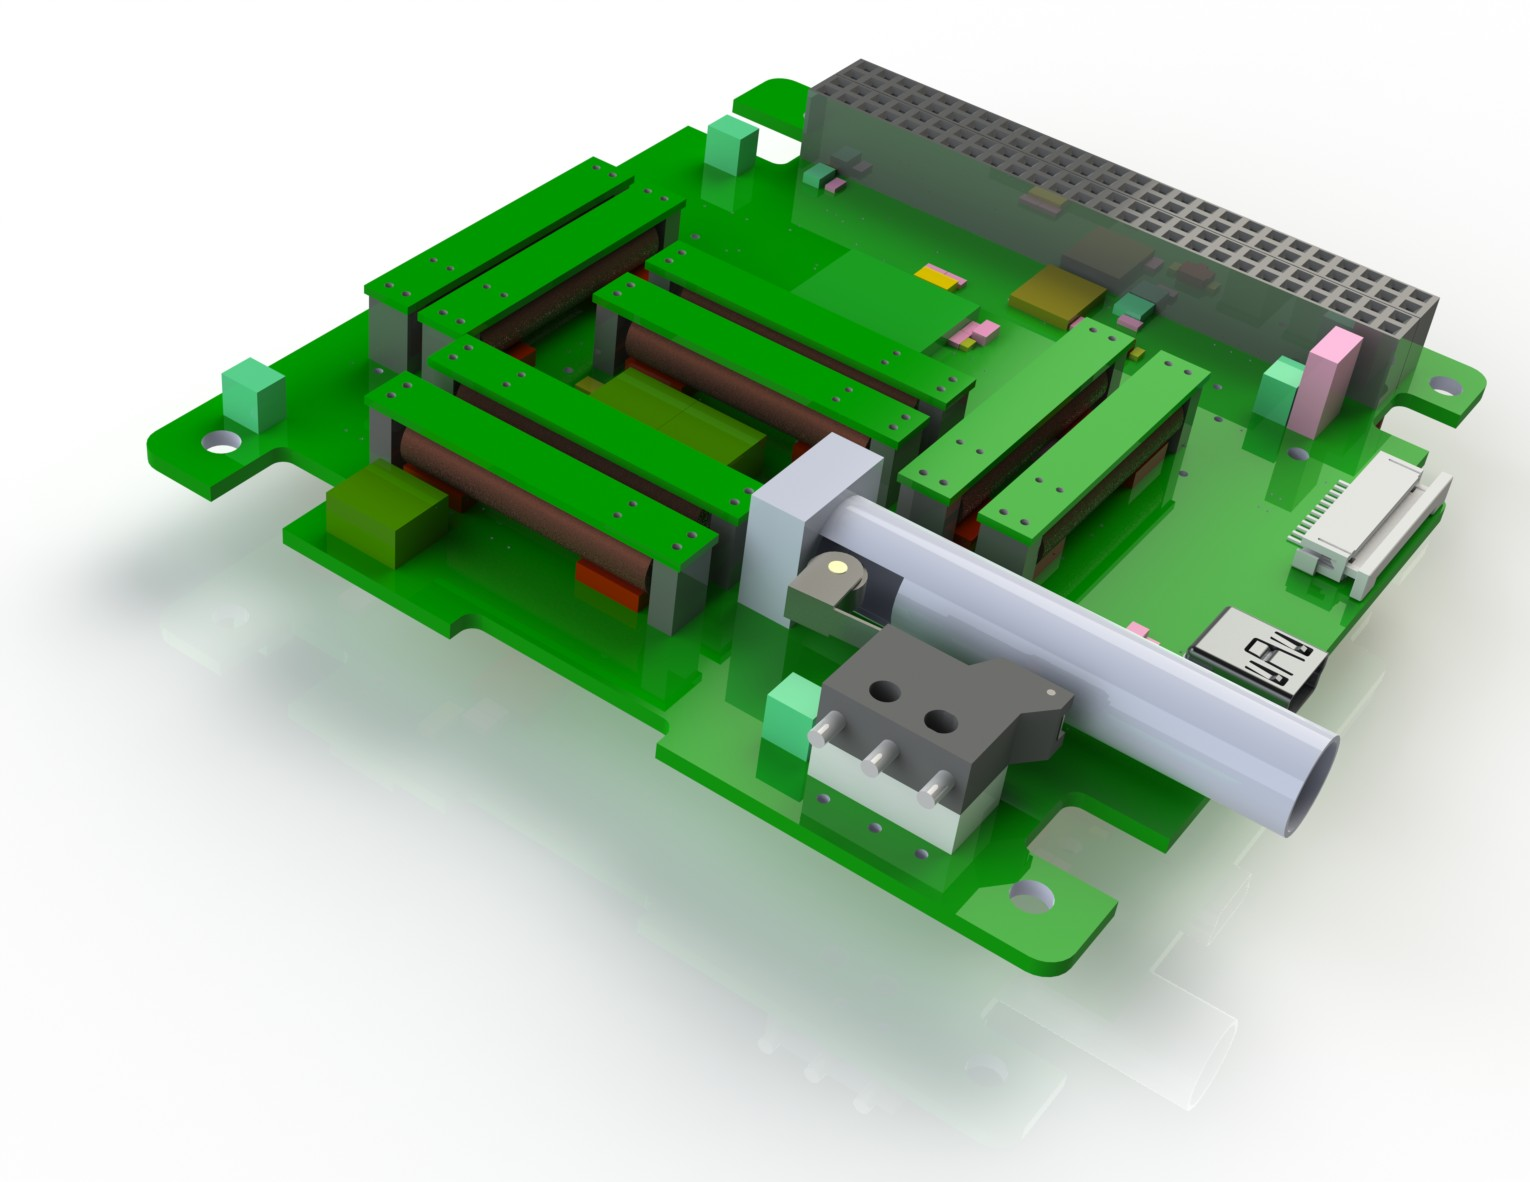
\includegraphics[width=0.8\textwidth]{board-drawing}
    \caption{3D view of the CubeSat \acs{ACDS} system}
    \label{fig:3dview}
\end{figure}

\begin{comment}
\begin{figure}[H]
    \centering
    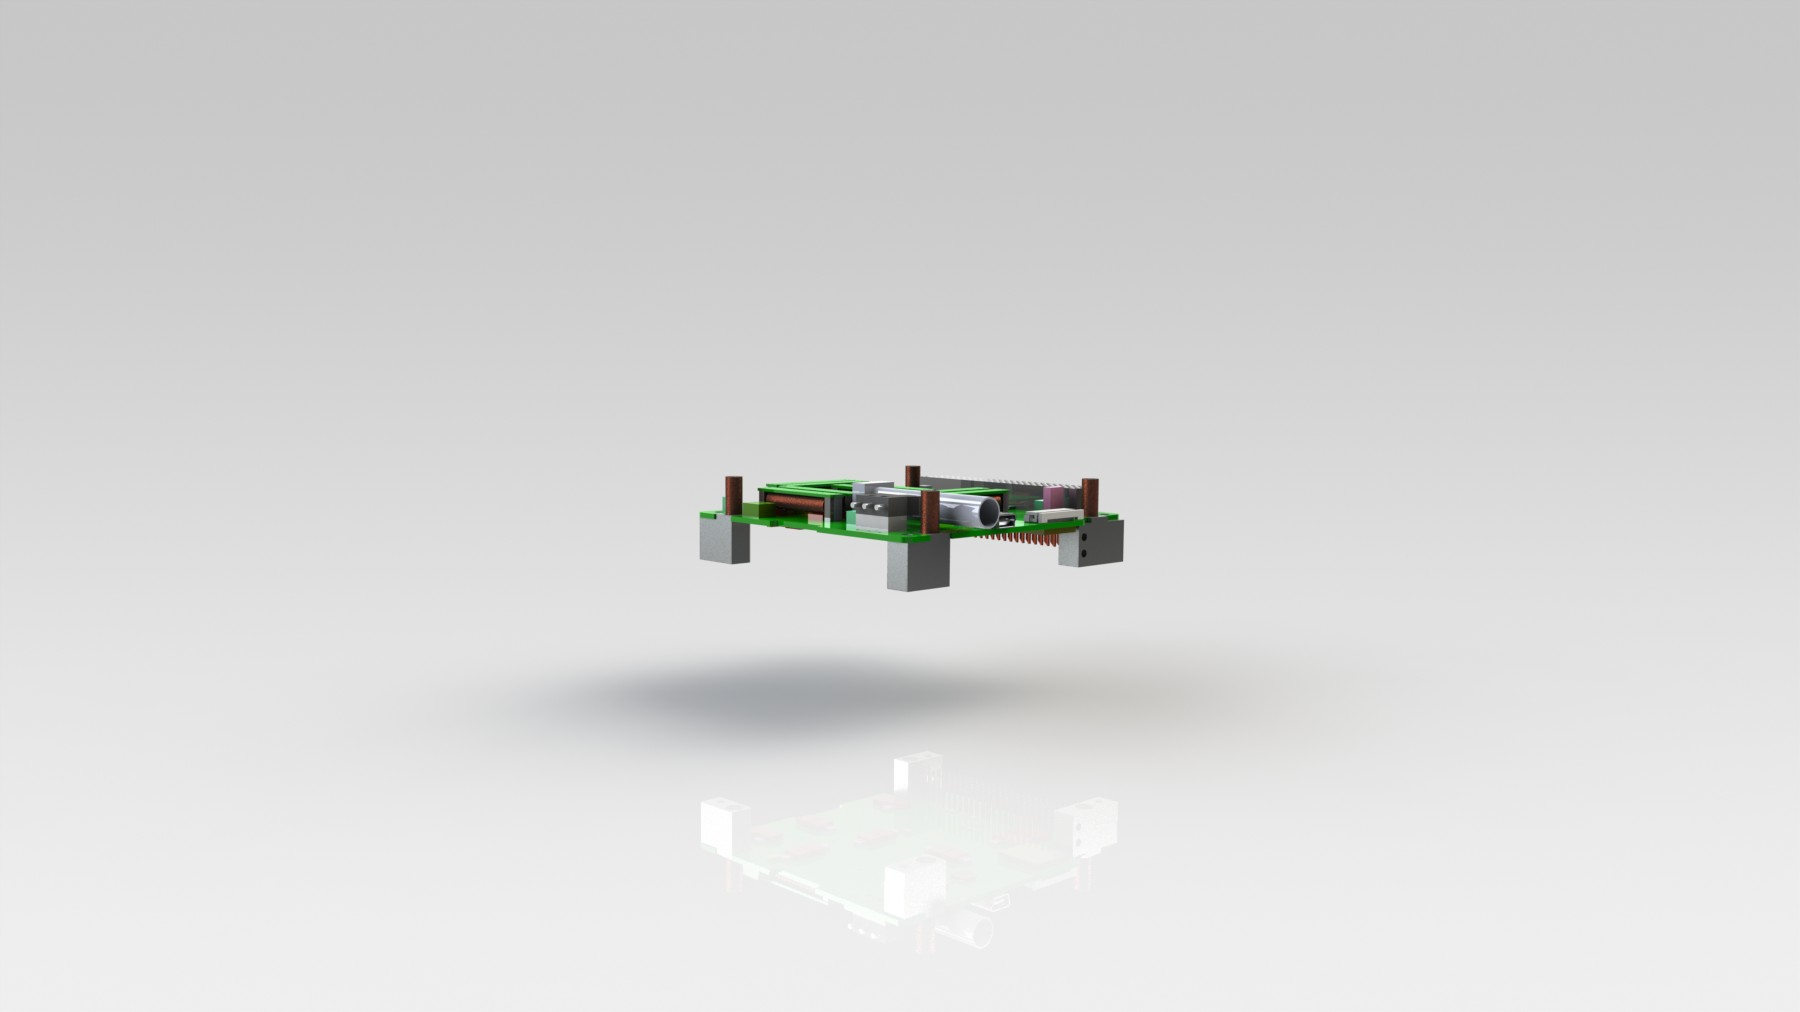
\includegraphics[width=0.8\textwidth]{board-drawing-with-standoffs}
    \caption{3D view of the CubeSat \acs{ACDS} system with Z-axis torquers}
\end{figure}
\end{comment}


The \ac{ACDS} board is a four layer board with the inner layers as power and ground planes. \Cref{fig:layout} shows the \ac{PCB} layout for the \ac{ACDS} board. The circuitry is very repetitive and this was used when the board was laid out. A quick switching time is desired and moderate currents are involved, the lines to and from the \acp{MOSFET} were kept as short as possible. The power plane is split so that there is a 3.3V plane underneath the MSP430 and a $V_{batt}$ plane elsewhere.

\begin{figure}[H]
    \centering
    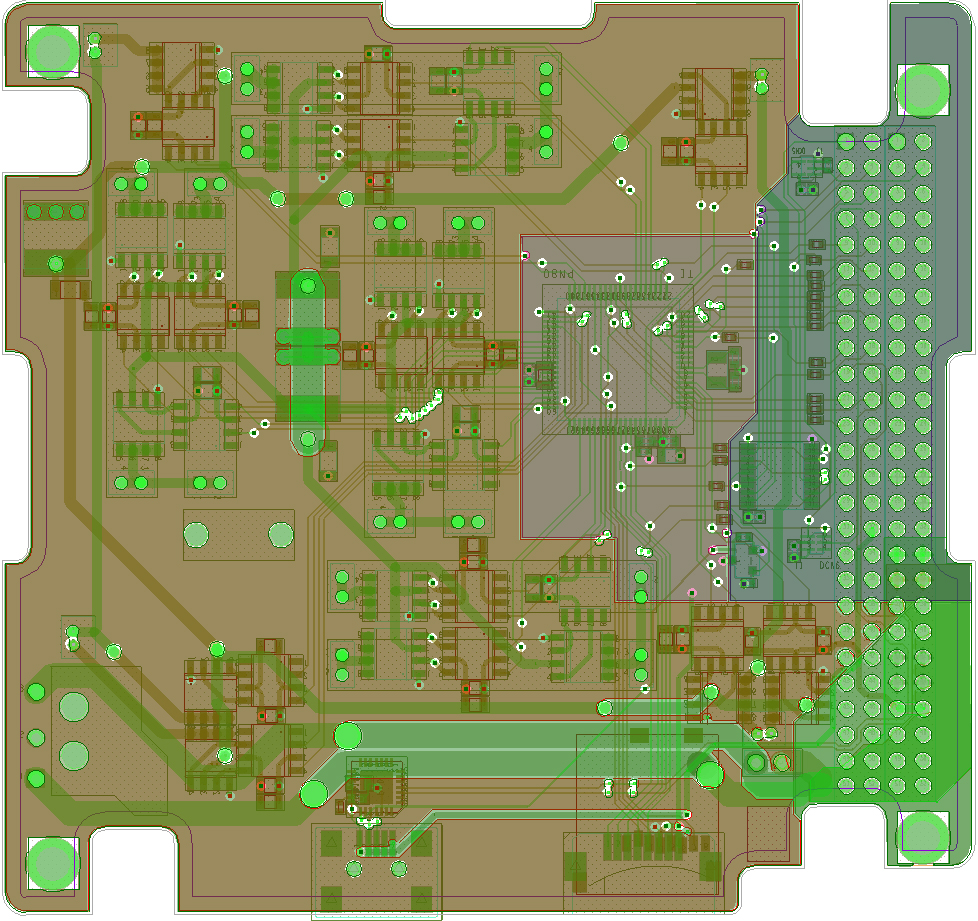
\includegraphics[width=0.8\textwidth]{board-design}
    \caption{Board Layout for the CubeSat \acs{ACDS} system}
    \label{fig:layout}
\end{figure}

